\documentclass[12pt]{report}
\usepackage{fontspec}
\usepackage[14pt]{extsizes}
\usepackage[english, russian]{babel} 
\defaultfontfeatures{Ligatures={TeX},Renderer=Basic} 
\setmainfont[Ligatures={TeX,Historic}]{Times New Roman}
\usepackage{setspace} % полуторный интервал

\usepackage{caption}

\usepackage{graphicx}
\usepackage[left=2cm, right=2cm, top=2cm, bottom=2.5cm]{geometry}
\usepackage{hyperref}
\usepackage{amsmath,amsfonts,amssymb,amsthm} 

\usepackage{titlesec, blindtext, color} % подключаем нужные пакеты
\definecolor{gray75}{gray}{0.75} % определяем цвет
\newcommand{\hsp}{\hspace{20pt}} % длина линии в 20pt
\titleformat{\chapter}[hang]{\Huge\bfseries}{\thechapter\hsp\textcolor{gray75}{|}\hsp}{0pt}{\Huge\bfseries}

\usepackage{listings}
% Для листинга кода:
\lstset{ 
	language=[Sharp]C,                 % выбор языка для подсветки (здесь это С)
	basicstyle=\small\sffamily, % размер и начертание шрифта для подсветки кода
	numbers=left,               % где поставить нумерацию строк (слева\справа)
	numberstyle=\tiny,           % размер шрифта для номеров строк
	stepnumber=1,                   % размер шага между двумя номерами строк
	numbersep=5pt,                % как далеко отстоят номера строк от подсвечиваемого кода
	showspaces=false,            % показывать или нет пробелы специальными отступами
	showstringspaces=false,      % показывать или нет пробелы в строках
	showtabs=false,             % показывать или нет табуляцию в строках
	frame=single,              % рисовать рамку вокруг кода
	tabsize=2,                 % размер табуляции по умолчанию равен 2 пробелам
	captionpos=t,              % позиция заголовка вверху [t] или внизу [b] 
	breaklines=true,           % автоматически переносить строки (да\нет)
	breakatwhitespace=false, % переносить строки только если есть пробел
}

\begin{document}
	
	%\def\chaptername{} % убирает "Глава"
	\begin{titlepage}
		\begin{table}[ht]
			\centering
			\begin{tabular}{|c|p{420pt}|} 
				\hline
				\begin{tabular}[c]{@{}c@{}} 
\includegraphics[scale=0.37]{source/EmblemBMSTU} \\\end{tabular} &
				\footnotesize\begin{tabular}[c]{@{}c@{}}\textbf{Министерство~науки~и~высшего~образования~Российской~Федерации}\\\textbf{Федеральное~государственное~бюджетное~образовательное~учреждение}\\\textbf{~высшего~образования}\\\textbf{«Московский~государственный~технический~университет}\\\textbf{имени~Н.Э.~Баумана}\\\textbf{(национальный~исследовательский~университет)»}\\\textbf{(МГТУ~им.~Н.Э.~Баумана)}\\\end{tabular}  \\
				\hline
			\end{tabular}
		\end{table}
		\noindent\rule{\textwidth}{4pt}
		\noindent\rule[14pt]{\textwidth}{1pt}
		\hfill 
		\noindent
		\makebox{ФАКУЛЬТЕТ~}%
		\makebox[\textwidth][l]{\underline{~~~~«Информатика и системы управления»~~~~~~~~~~~~~~~~~~~~~~~~~~~~~~~~~~~~~~~~~~~~}}%
		\\
		\noindent
		\makebox{КАФЕДРА~}%
		\makebox[\textwidth][l]{\underline{~~~~~~~«Программное обеспечение ЭВМ и информационные технологии»~~~~~~~~}}%
		\\
		
		
		\begin{center}
			\vspace{3cm}
			{\bf\huge Отчёт\par}
			{\bf\Large по лабораторной работе № 2\par}
			\vspace{0.5cm}
		\end{center}
		
		
		\noindent
		\makebox{\large{\bf Название:}~~~}
		\makebox[\textwidth][l]{\large\underline{~Алгоритмы умножения матриц~}}\\
		
		\noindent
		\makebox{\large{\bf Дисциплина:}~~~}
		\makebox[\textwidth][l]{\large\underline{~Анализ алгоритмов~}}\\
		
		\vspace{1.5cm}
		\noindent
		\begin{tabular}{l c c c c c}
			Студент      & ~ИУ7-55Б~               & \hspace{3.5cm} & \hspace{3.5cm}                 & &  Д.О. Склифасовский \\\cline{2-2}\cline{4-4} \cline{6-6} 
			\hspace{3cm} & {\footnotesize(Группа)} &                & {\footnotesize(Подпись, дата)} & & {\footnotesize(И.О. Фамилия)}
		\end{tabular}
		
		\vspace{1cm}
		
		\noindent
		\begin{tabular}{l c c c c}
			Преподователь & \hspace{6cm}   & \hspace{3.5cm}                 & & ~~~~~~ Л.Л. Волкова ~~~~~~\\\cline{3-3} \cline{5-5} 
			\hspace{3cm}  &                & {\footnotesize(Подпись, дата)} & & {\footnotesize(И.О. Фамилия)}
		\end{tabular}
		
		\begin{center}	
			\vfill
			\large \textit {Москва, 2020}
		\end{center}
		
		\thispagestyle {empty}
		\pagebreak
	\end{titlepage}
	\restoregeometry
	
	\tableofcontents
	\onehalfspacing
	\newpage
	\chapter*{Введение}
	\addcontentsline{toc}{chapter}{Введение}
	Цель работы: изучение алгоритмов умножения матриц. В данной лабораторной работе рассматриваются 3 алгоритма:
	\begin{enumerate}
		\item[1)] стандартный алгоритм умножения матриц;
		\item[2)] алгоритм Винограда;
		\item[3)] модифицированный алгоритм Винограда.
	\end{enumerate}
	\noindent Также требуется изучить рассчет сложности алгоритмов.
	В ходе лабораторной работы необходимо:
	\begin{enumerate}
		\item[1)] изучить алгоритмы умножения матриц;
		\item[2)] оптимизировать алгоритм Винограда;
		\item[3)] дать теоритическую оценку стандартного алгоритма умножения матриц, алгоритма Винограда и модифицированного алгоритма Винограда;
		\item[4)] реализовать три алгоритма умножения матриц на одном из языков программирования;
		\item[5)] сравнить алгоритмы умножения матриц.
	\end{enumerate}
	
	\newpage
	\chapter{Аналитическая часть}
	В данном разделе представлено математическое описание алгоритмов умножения матриц.
	
	\section{Стандартный алгоритм умножения матриц}
	Матрица — математический объект, записываемый в виде прямоугольной таблицы элементов кольца или поля (например, целых, действительных или комплексных чисел), которая представляет собой совокупность строк и столбцов, на пересечении которых находятся её элементы. Количество строк и столбцов задает размер матрицы. Хотя исторически рассматривались, например, треугольные матрицы, в настоящее время говорят исключительно о матрицах прямоугольной формы, так как они являются наиболее удобными и общими. 
	Умножение матриц — одна из основных операций над матрицами. Матрица, получаемая в результате операции умножения, называется произведением матриц.
	Пусть даны две прямоугольные матрицы A и B размером $[l * m]$ и $[m * n]$. В результате произведения матриц A и B получим матрицу $C$ размером $[l * n]$, в которой:
	\begin{equation}
		c_{i,j} = \sum_{r=1}^{m}a_{ir}b_{rj} \qquad (i=1,2,...l; j = 1,2,...n)
	\end{equation}
	Операция умножения двух матриц выполнима только в том случае, если число столбцов в первом сомножителе равно числу строк во втором; в этом случае говорят, что матрицы согласованы. В частности, умножение всегда выполнимо, если оба сомножителя — квадратные матрицы одного и того же порядка. 
	
	\section{Алгоритм Винограда}
	Если посмотреть на результат умножения двух матриц, то видно, что каждый элемент в нем представляет собой скалярное произведение соответствующих строки и столбца исходных матриц. Можно заметить также, что такое умножение допускает предварительную обработку, позволяющую часть работы выполнить заранее. \hyperref[literature]{[1]}\par
	Рассмотрим два вектора $V = (v_{1},v_{2},v_{3},v_{4})$ и $W = (w_{1},w_{2},w_{3},w_{4})$. Их скалярное произведение равно:
	\begin{equation}
		V * W = v_{1}w_{1} + v_{2}w_{2} + v_{3}w_{3} + v_{4}w_{4}
	\end{equation}
	Это равенство можно переписать в виде:
	\begin{equation}
		V * W = (v_{1} + w_{2})(v_{2} + w_{1}) + (v_{3} + w_{4})(v_{4} + w_{3}) -  v_{1}v_{2} - v_{3}v_{4} - w_{1}w_{2} - w_{3}w_{4}
	\end{equation}
	Менее очевидно, что выражение в правой части последнего равенства допускает предварительную обработку: его части можно вычислить заранее и запомнить для каждой строки первой матрицы и для каждого столбца второй. На практике это означает, что над предварительно обработанными элементами придется выполнять лишь первые два умножения и последующие пять сложений, а также дополнительно два сложения. 
	
	\section{Вывод}
	Было представлено математическое описание стандартного алгоритма умножения матриц и алгоритма Винограда. Основное отличие - наличие предварительной обработки, а также количество операций умножения.
	
	\newpage
	\chapter{Конструкторская часть}
	В данном разделе представлены схемы разработанных алгоритмов. Также оценивается трудоемкость алгоритмов.
	\section{Разработка алгоритмов}
	На \hyperref[Algorithm1]{рисунке 1} изображена схема стандартного алгоритма умножения матриц.
	\begin{figure}[h!]\label{Algorithm1}
		\center{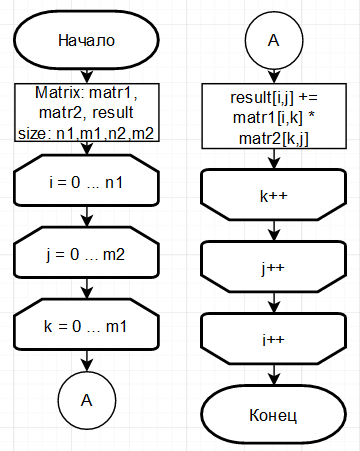
\includegraphics[scale=0.95]{source/Algorithm1.png}}
		\caption*{Рисунок 1. Схема стандартного алгоритма умножения матриц}
	\end{figure}
	\newpage
	На \hyperref[Algorithm2]{рисунке 2} изображена схема алгоритма Винограда.
	\begin{figure}[h!]\label{Algorithm2}
		\center{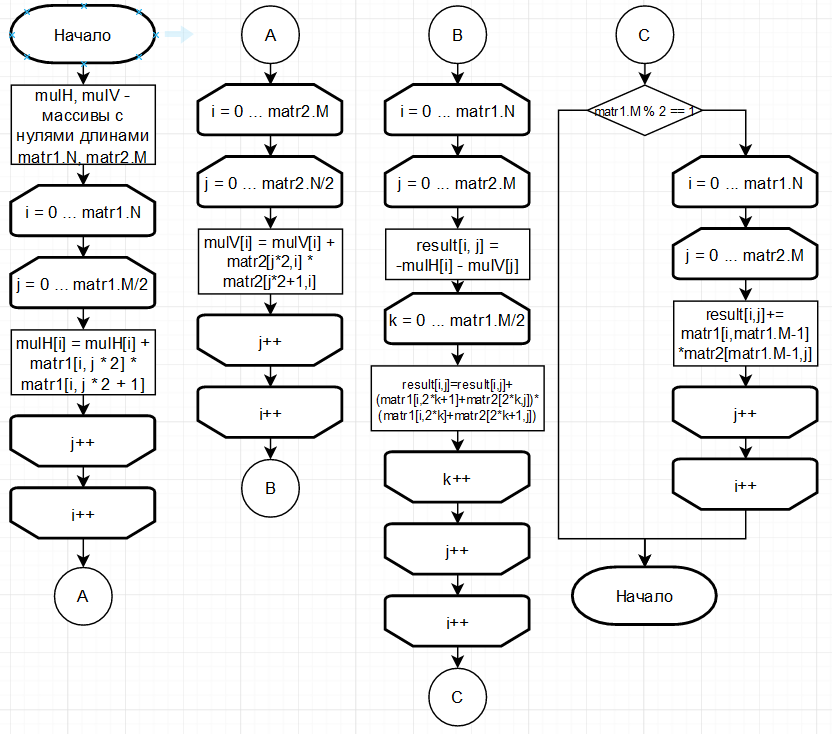
\includegraphics[scale=0.85]{source/Algorithm2.png}}
		\caption*{Рисунок 2. Схема алгоритма Винограда}
	\end{figure}
	\newpage
	На \hyperref[Algorithm3]{рисунке 3} изображена схема модифицированного алгоритма Винограда.
	\begin{figure}[h!]\label{Algorithm3}
		\center{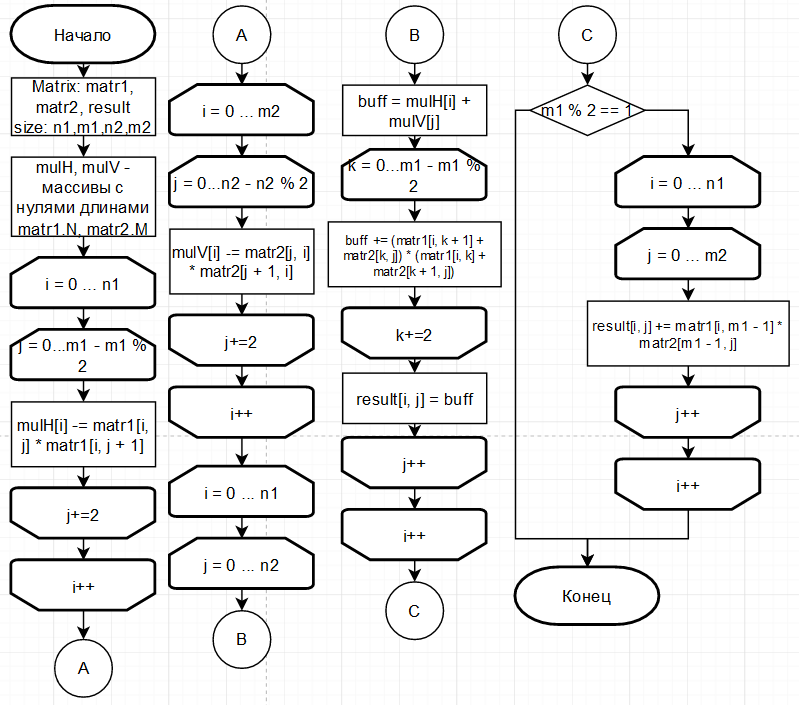
\includegraphics[scale=0.9]{source/Algorithm3.png}}
		\caption*{Рисунок 3. Схема модифицированного алгоритма Винограда}
	\end{figure}
	
	\newpage
	\section{Модель трудоемкости}
	Модель трудоемкости для оценки алгоритмов:
	\begin{enumerate}
		\item[1)] стоимость базовых операций единица:\par
		$=,+,*,\simeq,<,>,\geq,\leq,==,!=,[],+=,-=,*=,/=,++,--$;
		\item[2)] стоимость цикла:\par
		$f_{for}=f_{init}+f_{comp}+M(f_{body}+f_{increment}+f_{comp})$\par
		Пример: $for(i=0,i<M;i++){/* body */}$\par
		Результат: $2 + M(2+f_{body})$;
		\item[3)] стоимость условного оператора\par
		Пусть goto (переход к одной из ветвей) стоит 0, тогда\par
		\begin{displaymath}
			f_{f} = \left\{ \begin{array}{l l}
				min(f_{A},f_{B}), & \textrm{лучший случай}\\
				max(f_{A},f_{B}), & \textrm{худший случай}\\
			\end{array} \right.
		\end{displaymath}
		\item[4)] операция обращения к ячейки матрицы [i, j] имеет трудоёмкость равную двум.
	\end{enumerate}
	
	%\newpage
	\section{Трудоемкость алгоритмов}
	Оценим трудоемкости алгоритмов.
	\subsection{Трудоемкость предварительной проверки}
	\begin{table}[h]\label{table}
		\caption{Оценка веса}
		\begin{center}
			\begin{tabular}{|c c|} 
				\hline
				Код & Вес \\ [0.5ex] 
				\hline
				int n1 = matr1.N; & 2\\
				int n2 = matr2.N; & 2\\
				int m1 = matr1.M; & 2\\
				int m2 = matr2.M; & 2\\
				if ((m1 != n2) || n1 == 0 || n2 == 0) { return null; } & 5\\
				\hline
			\end{tabular}
		\end{center}
	\end{table}

	\subsection{Трудоемкость стандартного алгоритма}
	Подсчет: $1+1+n_{1}(2+1+1+m_{2}(2+1+1+m_{1}(2+8)))=2+n_{1}(4+m_{2}(4+m_{1}10))=2+n_{1}(4+4m_{2}+10m_{1}m_{2})=10n_{1}m_{1}m_{2}+4n_{1}m_{2}+4n_{1}+2$
	
	\subsection{Трудоемкость алгоритма Винограда}
	Подсчет:\par
	Первый цикл: $\frac{15}{2}n_{1}m_{1}+5n_{1}+2$\par
	Второй цикл: $\frac{15}{2}m_{2}n_{2}+5m_{2}+2$\par
	Третий цикл: $13n_{1}m_{2}m_{1}+12n_{1}m_{2}+4n_{1}+2$\par
	Условный оператор: 
	$\begin{bmatrix}
		2    &&, \text{невыполнение}\\
		15n_{1}m_{2} + 4n_{1} + 2 &&, \text{выполнение}\\
	\end{bmatrix} $ 
	
	Результат:	$13n_{1}m_{2}m_{1}+\frac{15}{2}n_{1}m_{1}+\frac{15}{2}m_{2}n_{2}+12n_{1}m_{2}+5n_{1}+5m_{2}+4n_{1}+6+$\par
	$\begin{bmatrix}
		2    &&, \text{невыполнение}\\
		15n_{1}m_{2} + 4n_{1} + 2 &&, \text{выполнение}\\
	\end{bmatrix} $

	\subsection{Трудоемкость модифицированного алгоритма Винограда}
	Подсчет:\par
	Первый цикл: $\frac{11}{2}n_{1}m_{1}+4n_{1}+2$\par
	Второй цикл: $\frac{11}{2}m_{2}n_{2}+4m_{2}+2$\par
	Третий цикл: $\frac{17}{2}n_{1}m_{2}m_{1}+9n_{1}m_{2}+4n_{1}+2$\par
	Условный оператор: 
	$\begin{bmatrix}
		2    &&, \text{невыполнение}\\
		10n_{1}m_{2} + 4n_{1} + 2 &&, \text{выполнение}\\
	\end{bmatrix}$\par
	Результат:
	$\frac{17}{2}n_{1}m_{2}m_{1}+\frac{11}{2}n_{1}m_{1}+\frac{11}{2}m_{2}n_{2}+9n_{1}m_{2}+8n_{1}+4m_{2}+6+$\par
	$\begin{bmatrix}
		2    &&, \text{невыполнение}\\
		10n_{1}m_{2} + 4n_{1} + 2 &&, \text{выполнение}\\
	\end{bmatrix}$
	
	\section{Вывод}
	В данном разделе были рассмотрены схемы алгоритмов умножения матриц, введена модель оценки трудоемкости алгоритма и были рассчитаны трудоемкости алгоритмов.
	
	\chapter{Технологическая часть}
	В данном разделе даны общие требования к программе, средства реализации и реализация алгоритмов.
	\section{Общие требования}
	\textbf{Требования к вводу:}
	\begin{enumerate}
		\item[1)] вводятся размеры матриц;
		\item[2)] вводятся (или автоматически генерируются) матрицы.
	\end{enumerate}
	\noindent\textbf{Требования к программе:}
	\begin{enumerate}
		\item[1)] при вводе неправильных размеров матриц программа не должна завершаться аварийно;
		\item[2)] должно выполняться корректное умножение матриц.
	\end{enumerate}
	
	\section{Средства реализации}
	В качестве языка программирования был выбран C\#,\hyperref[literature]{[2]} так как я знаком с данным языком программирования, имею представление о способах тестирования программы.\par
	Средой разработки Visual Studio.\hyperref[literature]{[3]}\par 
	Для замеров процессорного времени используется функция $Stopwatch$.\hyperref[literature]{[4]}
	
	\section{Сведения о модулях программы}
	Программа состоит из:
	\begin{enumerate}
		\item[1)] Program.cs - главный файл программы, в котором располагается точка входа в программу.
		\item[2)] Matrix.cs - файл класса Matrix. Класс реализует матрицу размером $n*m$, а также он содержит методы для работы с матрицами.
		\item[3)] Array.cs - файл класса Array. Класс реализует массив размером $n$, а также он содержит методы для работы с массивами.
		\item[4)] MultMatr.cs - файл класса MultMatr. В нем находятся алгоритмы умножения матриц.
	\end{enumerate}
	
	\section{Листинг кода программы}
	\begin{lstlisting}[label=Matrix,caption=Класс Matrix для работы с матрицами]
		class Matrix
		{
			private int n;
			private int m;
			private int[,] matrix;
			
			public Matrix() { }
			public Matrix(int n, int m)
			{
				this.n = n;
				this.m = m;
				matrix = new int[n, m];
			}
			
			public int N
			{
				get { return n; }
				set { if (value > 0) n = value; }
			}
			public int M
			{
				get { return m; }
				set { if (value > 0) m = value; }
			}
			
			public int this[int i, int j]
			{
				get { return matrix[i, j]; }
				set { matrix[i, j] = value; }
			}
			
			public void InputMatr()
			{
				for (int i = 0; i < n; i++)
				{
					for (int j = 0; j < m; j++)
					{
						Console.WriteLine("Введите эелемент матрицы {0}:{1}", i + 1, j + 1);
						matrix[i, j] = Convert.ToInt32(Console.ReadLine());
					}
				}
			}
			
			public void ReadMatr()
			{
				for (int i = 0; i < n; i++)
				{
					for (int j = 0; j < m; j++)
					{
						Console.Write(matrix[i, j] + "\t");
					}
					Console.WriteLine();
				}
			}
			
			public void FillMatr()
			{
				Random rand = new Random();
				for (int i = 0; i < n; i++)
				{
					for (int j = 0; j < m; j++)
					{
						matrix[i, j] = rand.Next(100);
					}
				}
			}
		}
	\end{lstlisting}
	\begin{lstlisting}[label=Array,caption=Класс Array для работы с массивами]
		class Array
		{
			private int[] array;
			private int n;
			public Array() { }
			
			public Array(int n)
			{
				this.n = n;
				array = new int[n];
			}
			
			public int N
			{
				get { return n; }
				set { if (value > 0) n = 0; }
			}
			
			public int this[int i]
			{
				get { return array[i]; }
				set { array[i] = value; }
			}
		}
	\end{lstlisting}
	\begin{lstlisting}[label=algorithm1,caption=Стандартный алгоритм умножения матриц]
		public static Matrix StandartMult(Matrix matr1, Matrix matr2)
		{
			int n1 = matr1.N;
			int n2 = matr2.N;
			int m1 = matr1.M;
			int m2 = matr2.M;
			if ((m1 != n2) || n1 == 0 || n2 == 0)
			{
				return null;
			}
			
			Matrix result = new Matrix(n1, m2);
			
			for (int i = 0; i < n1; i++)
			{
				for (int j = 0; j < m2; j++)
				{
					for (int k = 0; k < m1; k++)
					{
						result[i, j] += matr1[i, k] * matr2[k, j];
					}
				}
			}
			return result;
		}
	\end{lstlisting}
	\begin{lstlisting}[label=algorithm2,caption=Алгоритм Винограда]
		public static Matrix VinogradMult(Matrix matr1, Matrix matr2)
		{
			int n1 = matr1.N;
			int n2 = matr2.N;
			int m1 = matr1.M;
			int m2 = matr2.M;
			if ((m1 != n2) || n1 == 0 || n2 == 0)
			{
				return null;
			}
			
			Matrix result = new Matrix(n1, m2);
			Array mulH = new Array(n1);
			Array mulV = new Array(m2);
			
			for (int i = 0; i < n1; i++)
			{
				for (int j = 0; j < m1 / 2; j++)
				{
					mulH[i] += matr1[i, j * 2] * matr1[i, j * 2 + 1];
				}
			}
			for (int i = 0; i < n1; i++)
			{
				Console.WriteLine(mulH[i]);
			}
			for (int i = 0; i < m2; i++)
			{
				for (int j = 0; j < n2 / 2; j++)
				{
					mulV[i] += matr2[j * 2, i] * matr2[j * 2 + 1, i];
				}
			}
			for (int i = 0; i < m2; i++)
			{
				Console.WriteLine(mulV[i]);
			}
			for (int i = 0; i < n1; i++)
			{
				for (int j = 0; j < m2; j++)
				{
					result[i, j] = -mulH[i] - mulV[j];
					for (int k = 0; k < m1 / 2; k++)
					{
						result[i, j] += (matr1[i, 2 * k + 1] + matr2[2 * k, j]) * (matr1[i, 2 * k] + matr2[2 * k + 1, j]);
					}
				}
			}
			
			if (m1 % 2 == 1)
			{
				for (int i = 0; i < n1; i++)
				{
					for (int j = 0; j < m2; j++)
					{
						result[i, j] += matr1[i, m1 - 1] * matr2[m1 - 1, j];
					}
				}
			}
			
			return result;
		}
	\end{lstlisting}
	\begin{lstlisting}[label=algorithm3,caption=Модифицированный алгоритм Винограда]
		public static Matrix VinogradModMult(Matrix matr1, Matrix matr2)
		{
			int n1 = matr1.N;
			int n2 = matr2.N;
			int m1 = matr1.M;
			int m2 = matr2.M;
			if ((m1 != n2) || n1 == 0 || n2 == 0)
			{
				return null;
			}
			
			Matrix result = new Matrix(n1, m2);
			Array mulH = new Array(n1);
			Array mulV = new Array(m2);
			
			int smallerM = m1 % 2;
			for (int i = 0; i < n1; i++)
			{
				for (int j = 0; j < (m1 - smallerM); j += 2)
				{
					mulH[i] -= matr1[i, j] * matr1[i, j + 1];
				}
			}
			
			int smallerN = n2 % 2;
			for (int i = 0; i < m2; i++)
			{
				for (int j = 0; j < (n2 - smallerN); j += 2)
				{
					mulV[i] -= matr2[j, i] * matr2[j + 1, i];
				}
			}
			
			for (int i = 0; i < n1; i++)
			{
				for (int j = 0; j < m2; j++)
				{
					int buff = mulH[i] + mulV[j];
					for (int k = 0; k < (m1 - smallerM); k += 2)
					{
						buff += (matr1[i, k + 1] + matr2[k, j]) * (matr1[i, k] + matr2[k + 1, j]);
					}
					result[i, j] = buff;
				}
			}
			
			if (smallerM == 1)
			{
				for (int i = 0; i < n1; i++)
				{
					for (int j = 0; j < m2; j++)
					{
						result[i, j] += matr1[i, m1 - 1] * matr2[m1 - 1, j];
					}
				}
			}
			
			return result;
		}
	\end{lstlisting}
	
	\section{Вывод}
	В данном разделе были даны общие требования к программе, описаны средства реализации, были представлены сведения о модулях программы, а также реализованы три алгоритма умножения матриц (стандартный, Винограда, модифицированный винограда).
	
	\chapter{Экспериментальная часть}
	В данном разделе представлены результаты работы программы и приведен анализ времени работы кажого из алгоритмов.
	\section{Примеры работы программы}
	На \hyperref[Result1]{рисунке 4} представлен результат работы алгоритмов.
	\begin{figure}[h!]\label{Result1}
		\center{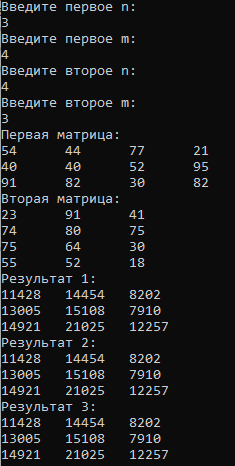
\includegraphics[scale=0.8]{source/Result1.png}}
		\caption*{Рисунок 4. Первый результат работы алгоритмов}
	\end{figure}
	\newpage
	На \hyperref[Result2]{рисунке 5} представлен результат работы алгоритмов.
	\begin{figure}[h!]\label{Result2}
		\center{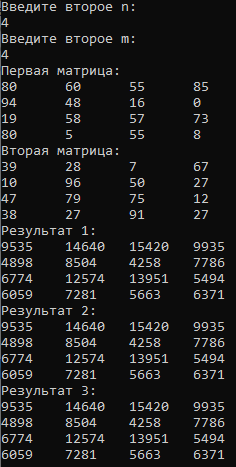
\includegraphics[scale=0.8]{source/Result2.png}}
		\caption*{Рисунок 5. Второй результат работы алгоритмов}
	\end{figure}

	\section{Анализ времени работы алгоритмов }
	Выполняется первый эксперимент при четном размере матриц. Берутся две матрицы размерами 100х100, 200х200, 300х300, 400х400, 500х500. Ячейки матрицы заполняются произвольно. Результат можно увидеть на \hyperref[Graphics1]{рисунке 6}.
	\begin{figure}[h!]\label{Graphics1}
		\center{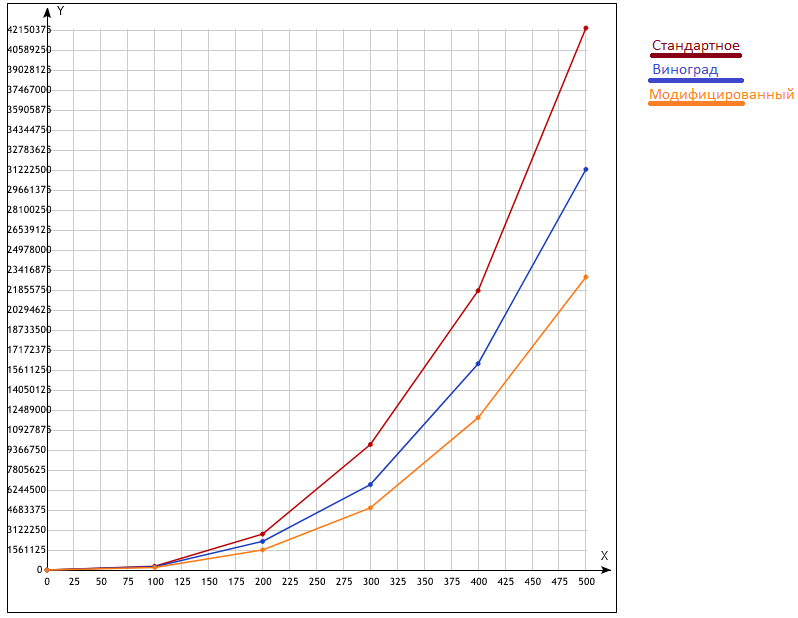
\includegraphics[scale=0.8]{source/Graphics1.png}}
		\caption*{Рисунок 6. Первый эксперимент для матриц с четными размерами}
	\end{figure} 
	\newpage
	\noindent Выполняется второй эксперимент при нечетном размере матриц. Берутся две матрицы размерами 101х101, 201х201, 301х301, 401х401, 501х501. Ячейки матрицы заполняются произвольно. Результат можно увидеть на \hyperref[Graphics2]{рисунке 7}.
	\begin{figure}[h!]\label{Graphics2}
		\center{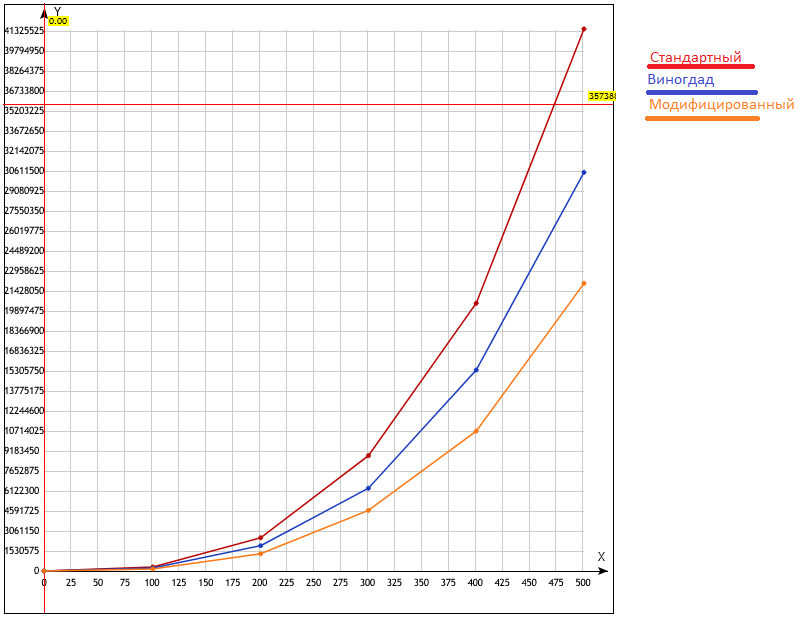
\includegraphics[scale=0.8]{source/Graphics2.png}}
		\caption*{Рисунок 6. Второй эксперимент для матриц с нечетными размерами}
	\end{figure} 
	\newpage
	
	\section{Вывод}
	Результаты тестирования показывают, что самым быстрым является модифицированный алгоритм Винограда. Самым медленным оказался стандартный алгоритм умножения матриц.

	\chapter*{Заключение}
	\addcontentsline{toc}{chapter}{Заключение}
	В ходе лабораторной работы были изучены алгоритмы умножения матриц: стандартный и Винограда. Также был модифицирован алгоритм Винограда. Были даны теоритические оценки алгоритмов умножения матриц. Была оценена трудоемкость алгоритмов. Также сравнили время работы алгоритмов, в результате которого стало понятно, что модифицированный алгоритм Винограда примерно в 2 раза быстрее, чем стандартный алгоритм и в 1.5 раза быстрее, чем алгоритм Винограда.

	\chapter*{Литература}
	\addcontentsline{toc}{chapter}{Литература}
	\begin{enumerate}
		\label{literature}
		\item Умножение матриц. -URL: \href{http://www.algolib.narod.ru/Math/Matrix.html}{http://www.algolib.narod.ru/Math/Matrix.html} (дата обращения: 11.10.2020). -Текст: электронный.
		\item  Документация по C\#. -URL: \href{https://docs.microsoft.com/ru-ru/dotnet/csharp/}{https://docs.microsoft.com/ru-ru/dotnet/csharp/} (дата обращения: 01.10.2020). -Текст: электронный.
		\item Документация по семейству продуктов Visual Studio. -URL:\par \href{https://docs.microsoft.com/ru-ru/visualstudio/?view=vs-2019}{https://docs.microsoft.com/ru-ru/visualstudio/?view=vs-2019 } (дата обращения: 01.10.2020). -Текст: электронный.
		\item Stopwatch Класс. -URL: \href{https://goo.su/2e99}{https://goo.su/2e99 } (дата обращения: 01.10.2020). -Текст: электронный.
		\item Под капотом у Stopwatch. -URL:  \href{https://habr.com/ru/post/226279/}{https://habr.com/ru/post/226279/} (дата обращения: 01.10.2020). Текст: электронный.
	\end{enumerate}

\end{document}

